% !TEX root = ../main.tex

\chapter{Design specification}\label{chap:design-spec}

\section{Customer requirements}

Through discussions with the project sponsor and analysis of the target application, eight customer requirements were identified and assigned importance weights reflecting the sponsor's priorities. The requirements capture both functional goals and non-functional concerns, including robustness, safety, generalizability, cost, and reliability.

\begin{table}[!htbp]
\centering
\caption{Customer requirements and importance weights}
\label{tab:cr}
\begin{tabular}{clc}
\toprule
\textbf{No.} & \textbf{Customer Requirement} & \textbf{Weight} \\
\midrule
CR1 & Complete assembly task successfully & 0.18 \\
CR2 & High assembly precision & 0.16 \\
CR3 & Robust to environment and disturbances & 0.15 \\
CR4 & Safe and collision-free operation & 0.14 \\
CR5 & Fast task execution & 0.12 \\
CR6 & Easy to use and generalize & 0.10 \\
CR7 & Cost-effective system & 0.08 \\
CR8 & System reliable and recovery capable & 0.07 \\
\bottomrule
\end{tabular}
\end{table}

The customer requirements were translated into engineering specifications through the QFD process rather than by assigning targets independently. For each customer requirement $i$ and engineering specification $j$, the team assigned a relationship value $r_{ij}\in\{0,1,3,9\}$ (none, weak, moderate, or strong) and calculated the unnormalized engineering priority as
\begin{equation}
I_j=\sum_i w_i r_{ij},
\end{equation}
where $w_i$ is the customer-importance weight in Table~\ref{tab:cr}. The priorities were then normalized to identify the technical characteristics that most directly protect the high-weight needs. CR1 and CR5 primarily drive ES1 and ES2; CR2 drives ES3 and ES4; CR3, CR4, and CR8 drive ES5 and ES6; and CR6--CR7 constrain the selected implementation to a usable, feasible, and maintainable route. This translation produces an auditable chain from the sponsor's language to acceptance tests and explains why the later concept search is organized around platform, teleoperation, data collection, gripper, and policy modules.

\section{Engineering specifications}

The customer requirements were converted into six measurable engineering specifications. The targets in Table~\ref{tab:es} are the final acceptance thresholds for the present proof-of-concept, rather than performance claims. Each rate is calculated over independently initialized physical trials of the relevant task. A trial is counted once only; an unsuccessful recovery is not reclassified as an independent execution attempt. This convention prevents recovery behavior from artificially inflating the reported task-execution success rate.

\begin{table}[!htbp]
\centering
\caption{Final engineering specifications and acceptance thresholds}
\label{tab:es}
\small
\begin{tabularx}{\textwidth}{
  >{\centering\arraybackslash}p{0.06\textwidth}
  p{0.18\textwidth}
  >{\centering\arraybackslash}p{0.10\textwidth}
  X}
\toprule
\textbf{No.} & \textbf{Engineering Specification} & \textbf{Target} & \textbf{Operational Definition} \\
\midrule
ES1 & Planning success rate & $>90\%$ & Fraction of trials in which the selected task policy and initialized scene form a valid executable plan. \\
ES2 & Task execution success rate & $>70\%$ & Fraction of trials in which the prescribed assembly operation reaches its task-specific completion condition. \\
ES3 & Component detection accuracy & $>90\%$ & Fraction of evaluated observations in which the required component is correctly detected for the active task. \\
ES4 & Pose estimation error & $<20$\,mm & Terminal pose error relative to the task-specific reference pose, evaluated as a binary threshold from the completion geometry. \\
ES5 & Failure detection rate & $>90\%$ & Fraction of induced or naturally occurring execution failures that are identified before further unsafe action is issued. \\
ES6 & Recovery rate & $>70\%$ & Fraction of detected failures for which the defined recovery procedure restores a valid task state. \\
\bottomrule
\end{tabularx}
\end{table}

ES4 retains the project term \emph{pose estimation error}. Conceptually, its
translational component is
\begin{equation}
e_{\mathrm{pose}}=\left\lVert \hat{\mathbf p}-\mathbf p_{\mathrm{ref}}\right\rVert_2,
\label{eq:es4-pose-error}
\end{equation}
where \(\hat{\mathbf p}\) denotes the terminal component position assessed by
the task geometry and \(\mathbf p_{\mathrm{ref}}\) is the task-specific
reference position. The final protocol evaluates only whether
\(e_{\mathrm{pose}}<20\)~mm; it does not log a continuous millimetre value.
For each of the three tasks, the fixture and accepted terminal region are
defined so that completion is not possible when
\(e_{\mathrm{pose}}\geq20\)~mm. A successful terminal state is therefore
recorded as zero threshold violation, not as a measured error of exactly
0~mm. A failed trial does not reach the terminal state to which ES4 applies
and is recorded as not applicable for ES4. Chapter~\ref{chap:validation}
applies this rule to 25 trials per task: 75 attempts produced 59
ES4-evaluable terminal states and 16 non-terminal outcomes.

\section{Quality function deployment}

Figure~\ref{fig:qfd} records the resulting House of Quality. Its 9--3--1 relationship scale makes the engineering priorities interpretable rather than decorative: task completion, component localization, pose estimation, and failure handling carry influence across multiple high-weight customer requirements. The roof is used as a design-control device. For example, additional visual coverage can strengthen ES3 and ES4, but it increases calibration, synchronization, and data-management burden; similarly, recovery logic can improve ES5--ES6 while adding controller integration work. These QFD trade-offs define the subsequent concept space. The platform and gripper must enable precise contact motion for ES1--ES2 and ES4; the teleoperator and data pipeline must produce usable demonstrations and observable scenes; and the policy must convert those observations into safe executable actions while leaving explicit hooks for failure monitoring and recovery.

\begin{figure}[!htbp]
\centering
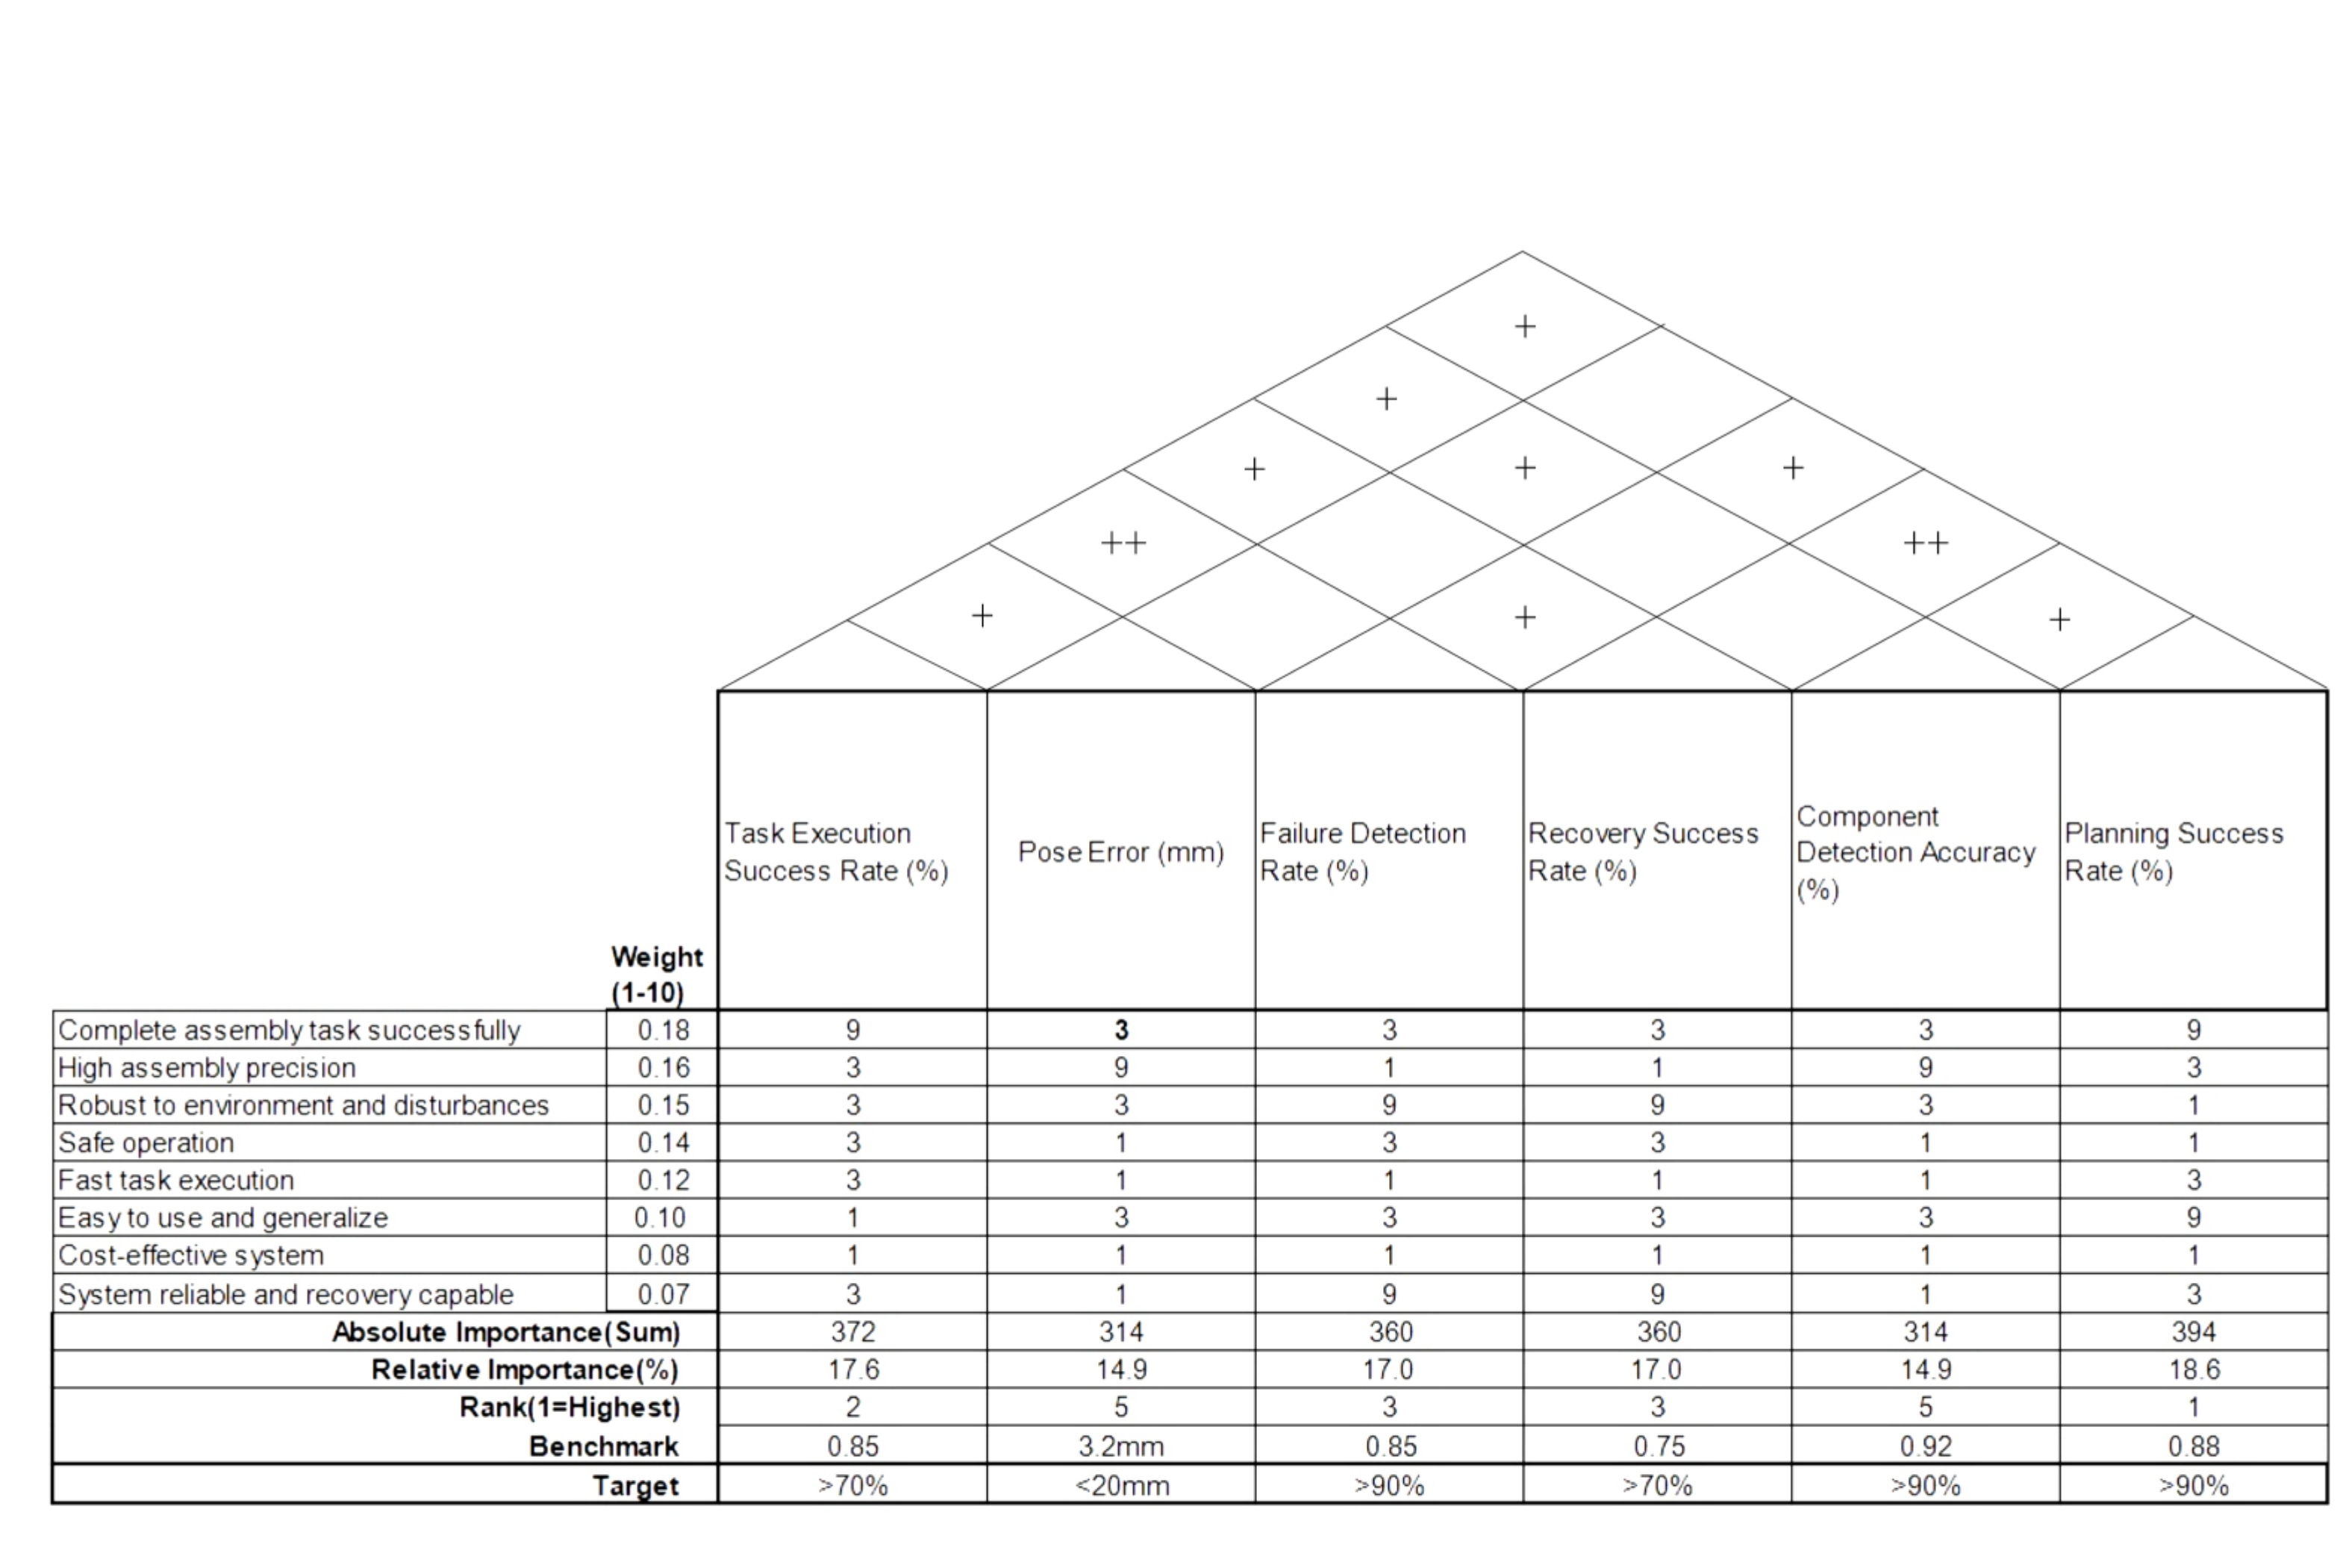
\includegraphics[width=0.95\textwidth]{qfd.jpg}
\caption{QFD House of Quality for the VLA bimanual manipulation system.}
\label{fig:qfd}
\end{figure}
